%-----------------------------------------------------
% index key words
%-----------------------------------------------------
\index{volume!oblique cylinder}
\index{volume}
\index{oblique cylinder}
%-----------------------------------------------------
% name, leave blank
% title, if the exercise has a name i.e. Hilbert's matrix
% difficulty = n, where n is the number of stars
% origin = "\cite{ref}"
%-----------------------------------------------------
\begin{Exercise}[
name={},
title={}, 
difficulty=0,
origin={\cite{YL}}]
A cylinder where the sides are not perpendicular to the base (the circle) is called an \emph{oblique cylinder}.
Given the oblique cyclinder defined by the given vectors $\vec{u}=(2,2,4),\; \vec{v}=(1,2,1)$ and $\vec{w}=(4,1,3)$.  Find the volume of the oblique cylinder.
\begin{multicols}{2}
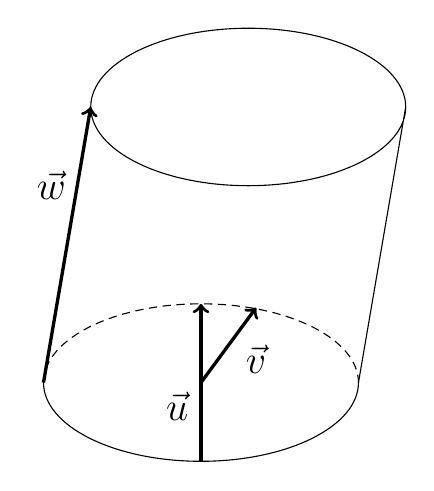
\begin{tikzpicture}

\pgfmathsetmacro{\cylinderradius}{2}
\pgfmathsetmacro{\cylinderheight}{3.5}
\pgfmathsetmacro{\aspectratio}{1}
\pgfmathsetmacro{\opacitycolor}{0}
\pgfmathsetmacro{\dx}{0.6}

%\fill[  left color=gray!70,
%             right color=gray!70,
%            middle color=gray!40,
%            shading angle=79,
%            opacity=\opacitycolor] (\cylinderradius,0) -- (\cylinderradius+\dx,\cylinderheight) arc (360:180:\cylinderradius*1cm and \aspectratio*1cm) -- (-\cylinderradius,0) arc (180:0:\cylinderradius*1cm and \aspectratio*1cm);
% Bottom fill:
%\fill[   top color=gray!95,
%            middle color=gray!70,
%            bottom color=gray!40,
%            opacity=\opacitycolor] (0,0) circle (\cylinderradius*1cm and \aspectratio*1cm);
% Top fill:
%\fill[   top color=gray!70,
%            middle color=gray!40,
%            bottom color=gray!10,,
%            opacity=\opacitycolor] (0+\dx,\cylinderheight) circle (\cylinderradius*1cm and \aspectratio*1cm);
% Cylinder lines:
\draw (-\cylinderradius+\dx,\cylinderheight) -- (-\cylinderradius,0) arc (180:360:\cylinderradius*1cm and \aspectratio*1cm)
        -- (\cylinderradius+\dx,\cylinderheight) ++ (-\cylinderradius,0) circle (\cylinderradius*1cm and \aspectratio*1cm);

\draw[<-, very thick] (-\cylinderradius+\dx,\cylinderheight) -- (-\cylinderradius,0);
\draw (-1.9,2.5) node{\Large$\vec{w}$};
\draw (-0.3,-0.3) node{\Large$\vec{u}$};
\draw (0.7,0.3) node{\Large$\vec{v}$};
% Dashed line in the back:
\draw[densely dashed] (-\cylinderradius,0) arc (180:0:\cylinderradius*1cm and \aspectratio*1cm);
\draw[->, very thick] (0,-1) -- (0,1);
\draw[->, very thick] (0,0) -- (0.7,0.95);

\end{tikzpicture}
Note from the diagram that $\vec{w}$ is not perpendicular to the base,
that $\vec{v}$ is positioned such that its tail is at the center of the circle and its tip lies on the circle,
that $\vec{u}$ is positioned such that the vector passes through the center of the circle while its tail and tip lie on the circle.
\textit{(Hint: the volume of an oblique cyclinder is equal to the area of the base times the height.)}
\EndCurrentQuestion
\end{multicols}
\end{Exercise}

\begin{Answer}
$\frac{48\pi\sqrt{11}}{11}$
\end{Answer}
